%\documentclass{article}
\documentclass[letterpaper,twocolumn,11pt]{article}
\usepackage[margin=0.75in]{geometry}
\usepackage{color}
\usepackage[hyphens]{url}
\usepackage{graphicx}
\usepackage{enumitem}
\usepackage{pdfpages}

\def\etal{{\it et al.~}}
\newenvironment{packed_enum}{
\begin{enumerate}
  \setlength{\itemsep}{1pt}
  \setlength{\parskip}{0pt}
  \setlength{\parsep}{0pt}
}{\end{enumerate}}
\newenvironment{packed_item}{
\begin{itemize}
  \setlength{\itemsep}{1pt}
  \setlength{\parskip}{0pt}
  \setlength{\parsep}{0pt}
}{\end{itemize}}

\begin{document}

\title{Assessing Tor's Usability as a Censorship Circumvention Tool}
\author{Linda N. Lee, David Fifield\\
University of California, Berkeley, \{lnl, fifield\}@cs.berkeley.edu
}
\maketitle
 
\begin{abstract}
\indent \indent Tor has grown beyond its original purpose of anonymity
to become an important tool for
Internet censorship circumvention.
We describe an experiment to assess the usability of Tor Browser,
a web browser with a bundled Tor proxy,
for the purpose of circumvention.
We focus our analysis on the browser's connection configuration dialog,
which enables circumvention even under stringent censors,
when used correctly.
The experiment is aimed at evaluating whether, and how easily users can circumvent censorship using Tor Browser,
under several censorship environments.
We present the design of the experiment,
which will involve hundreds of users completing seven browsing tasks in three different adversarial settings.
We describe the results of a smaller-scale pilot study,
the lessons we learned from it,
and how it guided our future experimental ambitions.
The experiment we describe is scheduled to run in August 2015.
\end{abstract}

\section{Introduction}

\indent \indent We aim to improve user security by evaluating
and improving the usability of security software.
Both ``usability'' and ``security'' encompass many topics;
therefore we limit our scope and focus on
an important and timely use case:
user configuration of software to evade Internet censorship.
In this report, we detail the design of a usability-focused user experiment,
which we hope will be a benchmark for such studies
and guide their development in the future.

We hold that usability must be regarded as a security property.
It should be part of the design of security software.
Usable software not only decreases the risk of making mistakes
with dangerous security consequences,
but also provides a bridge over which users can
transition from substitutes that are less safe.

The heart of our investigation will be a large-scale user study
that measures how effectively users are able to complete
basic web browsing tasks in the presence of a censor.
We will place users in a controlled network environment
that simulates the kind of censorship conditions that many
users around the world face daily.
We will be testing specific circumvention software---namely,
Tor Browser---though our larger contribution is to establish
a usability testing methodology for the evaluation
of this kind of software.

\subsection{Censorship} %%%
% \indent \indent Motivational paragraph time about how this is so everywhere. 

\indent \indent Censorship and other information controls
are widespread on the Internet and increasing in prevalence.
Since 2011, Freedom House has published a yearly report
on the state of Internet freedom in dozens of countries.
The 2014 report~\cite{freedom-on-the-net-2014} observes
an overall decrease in freedom worldwide,
with 36 of 65 surveyed countries decreasing in their freedom rating
since 2013 (only 12 countries had an increase).

To escape restrictive networks and communicate more freely,
users turn to a variety of censorship circumvention technologies.
What tools are necessary depends greatly on the specifics of
a particular censor;
they range from simple one-hop proxies and VPNs
to complicated steganographic systems.
Our goal is the development of an experiment
to test the usability of such tools.
We focus on one particular system,
Tor Browser, which bundles a variety of circumvention
tools designed for different use cases.

\subsection{Tor} 

\indent \indent The Tor Project, known for its anonymity network~\cite{tor-design},
has in recent years become an important player in the world of
censorship circumvention.
In its early days, people used Tor to evade censorship,
and in response censors began to block Tor itself.
In response, work began on various anti-censorship technologies
now known as ``pluggable transports''~\cite{pluggable-transports}.
Currently there are over 15,000 users accessing the Tor network
at any given time using one of these
anti-censorship technologies~\cite{userstats-bridge-country}.

Tor Browser~\cite{tor-browser},
a specially modified version of Firefox that comes
with a built-in Tor proxy and pluggable transports,
is the primary means through which users access the Tor network.
It aims to make powerful anonymity and circumvention technology
accessible even to nontechnical users.
Its user interface was greatly overhauled in its version~3.5 release,
and since then it has not had a comprehensive usability evaluation.

\subsection{What is Required of Users}
\indent \indent For users to circumvent censorship in their resident countries, they will need to 
configure Tor to set up a proxy, bridge, or both. The requirement of the user will vary on their censorship
environment, specifically, if they need to conceal the fact that they are using Tor or if Tor entry nodes 
have been blocked by the government. There is a configuration wizard to help guide users through setting up their connection, but they require the user to provide IP addresses of proxies or bridges to use.

The end user generally does not care about the details of the 
censorship environment, and how the censorship is implemented; rather, they care about how to get
to the website of their choice. In the wild, users may choose to get the required information in a variety 
of ways, including reading online manuals on how to configure Tor, finding out information through word of mouth, 
or figuring out correct configurations themselves by trial and error.  We cannot accurately simulate the effects
of these localized effects during our experiment.

However, we are testing the usability, and therefore comprehension and user-friendliness, of the Tor configuration 
dialog, which will require users in the most strict censorship environments to navigate through three configuration windows and provide correct answers all along the process in order to configure the connection correctly. Knowledge
required includes if their connection would require a proxy to access the Internet, the IP address of a bridge if required, 
and which pluggable transports are functional in their country. 

\section{A Pilot Tor Usability Study} 
\indent \indent We ran a pilot Tor usability study to test the usability of Tor as an anonymity tool,
targeting a specific demographic of users known to use Tor (journalists who have reported in other
countries) and aiming to identify how well they could understand Tor's non-typical behaviors and 
navigate advanced settings. For the full details of this pilot experiment, we refer you to Appendix ~\ref{sec:pilot}.  

During this pilot, the users were struggling with confusing bugs, such as flash errors which
say ``Firefox'' rather than ``Tor,'' disappearing buttons on the configuration window, and errors when
launching Tor from the download dialog rather than from their applications folder. This resulted in our 
participants spending most of their time on the download and install tasks, rather than 
our original task for navigating a robust menu or questioning the clarity of provided security 
guarantees. We took the opportunity to collaborate with Tor developers to make changes for the Tor 
Browser and use the lessons learned to design our large-scale user study on testing Tor as a 
censorship circumvention tool. 

\subsection{Impact}
\indent \indent Along with the Tor developers who came to observe the UX pilot, we filed 
a total of sixteen bug tickets to Tor. At the time of  this writing, eight of the sixteen tickets 
have already been resolved, and more will be resolved in the future.  The list of bug
tickets filed can be found at \url{https://trac.torproject.org/projects/tor/query?keywords=~uxsprint2015}. 

As of April, the changes resulting from our pilot study has been incorporated into the latest 
version of Tor Browser, making Tor more usable for people to use. 
The summary of the usability changes can be found at \url{https://blog.torproject.org/blog/tor-browser-45a4-released}. 

Through the publicity of this usability pilot study on the Tor weekly blogs, we were connected
with a source from the Library Freedom Project, which provides training on various technologies 
to libraries across the country. We now collaborate with her work on creating a user manual
for the Tor Browser. 

\subsection{Lessons Learned} 
\indent \indent During the pilot study, we were attempting to test out a comprehensive set of 
features for the Tor Browser. Our users had difficulties completing all the given tasks in the 
time allotted for the experiment. Additionally, user fatigue was very evident, with users not 
engaging in the later set of tasks after being tired from the download and install process. 
To ensure that the experiment does not cause user fatigue, we select a smaller set of features 
as the target for the full-scale study.  After deliberating with Tor developers, and testing out
various features on our own, we chose to focus on the Tor Browser connection configuration 
dialog because of its crucial role in censorship circumvention. 

Although the data from the pilot study provided a lot of insight into what users thought processes
are when completing various asks, transcribing audio recordings and syncing them to videos was
required a lot of manual labor. Not only did this form of data collection and processing not scale 
to larger numbers, we found that most users encountered similar thought processes and struggled
with the same issues. Because of this, we aim to collect our future qualitative data in the form of 
an open-ended survey question rather than using audio recordings. 

\section{Experiment Design}

\subsection{Assumptions} 
{\color{red} do I need this here?}

\subsection{Overview} 
Our experiment consists of three parts: informing and motivating the participants in order 
to roleplay in the experiment, asking our participants to complete a set of web browsing tasks which will 
require them to circumvent censorship using the Tor Browser, and soliciting feedback from our participants
about their experience. With participants' consent, we will also record their computer screen to monitor 
their activity and employ a browser extension to take empirical measurements (such as idle waiting time, 
or how fast a particular task was completed) throughout the duration of this experiment. 

Each session of 30 participants will be placed in the same simulated censorship environment. 
We start off the experiment by informing our participants that they are in an adversarial setting, 
where some websites are blocked while other websites are not. We will instruct them to visit a censored
website and a non-censored website to illustrate that their devices and the network is fully functional and
operating as expected, but that they are in a censorship environment where some websites will fail to load. 
We will take a moment to explain what Tor is, how it is generally used in this case, and ask them to complete 
the aforementioned set of tasks. To complete all the tasks, the participants will ultimately need to get the correct
configuration settings for the country they are simulated to be in.  Figure ~\ref{dialog} shows one of the 
Tor configuration dialog screens that a user will need to navigate. 

Then, each participant will be given about 30 minutes to complete their given Internet browsing tasks. 
Note that these Internet tasks themselves do not take very much time, but that the time is allotted in order
for participants to complete the configuration process. We believe that this is more than enough time to 
test the usability of the configuration process. Even if some participants may have succeeded with more 
time, we consider these cases to be a failure from a usability perspective as this would require too much
time from a user in the wild. Minimal interaction will be allowed with participants and the researchers. 
Researchers may inform participants of specific information (such as a bridge address) in a manner 
which does not disturb other participants (such as instructing users to visit a specific non-blocked website 
containing this information). 

We will end the experiment with a survey of 17 questions in order to collect basic participation information, 
demographics of our participants, open-ended responses of their experience with censorship circumvention,
and general security questions to gauge their awareness in this area. Along with the empirical measurements 
we have taken during the experiment, we will use this survey information to determine which configuration tasks are hard (bridges versus proxies, etc.), how many were successful, how long it took users to configure, if they understood the process, if they were confident that it was working as expected, etc.  

\subsection{Censorship Environment Simulation}

\begin{figure}[t]
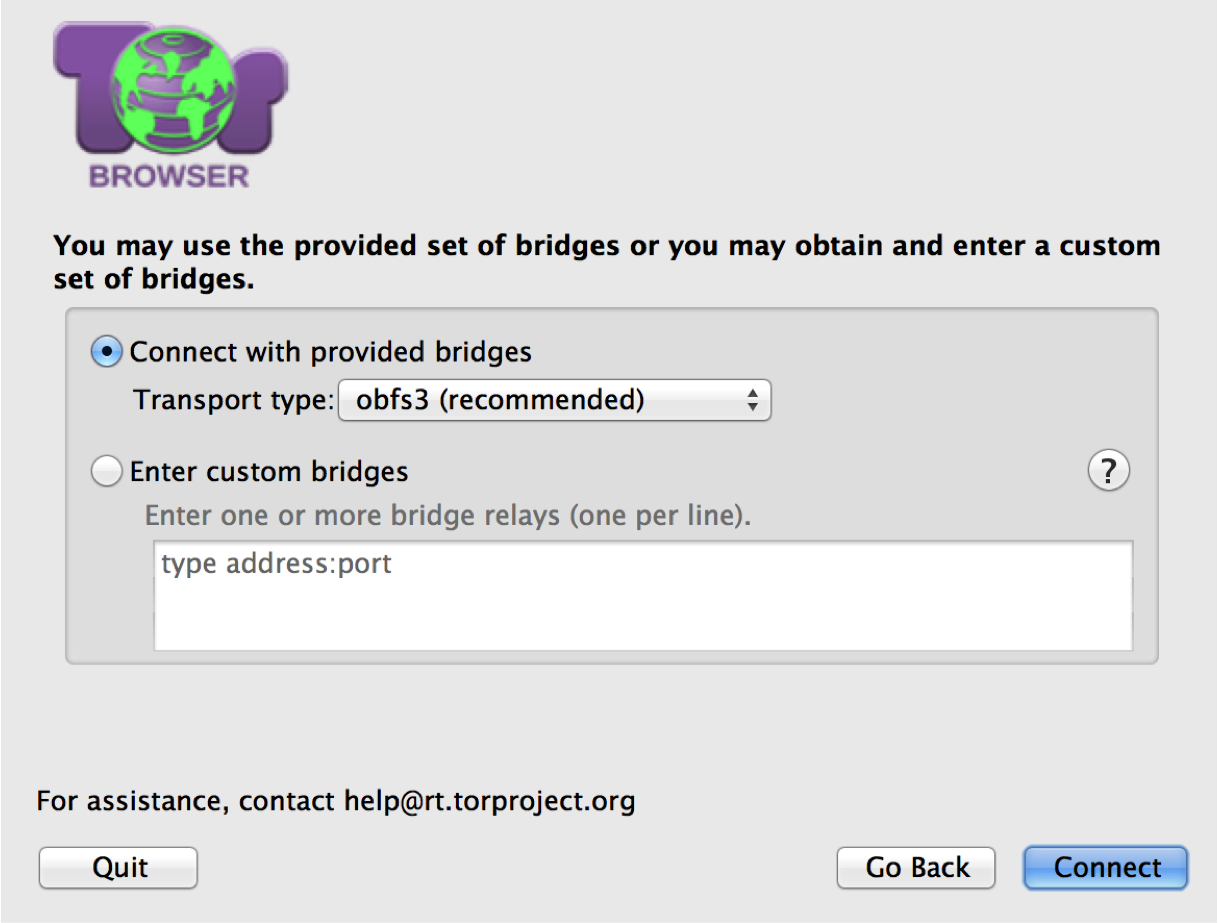
\includegraphics[width=\linewidth]{configuration-dialog.png}
\caption{The fourth and final window of the Tor configuration dialog is what users will use to 
configure their network settings to circumvent censorship. The instructions asks users to 
choose a pluggable transport or enter custom bridges.}
\label{dialog}
\end{figure}

\indent \indent For our experiment, we plan to simulate and test three distinct censorship environments
which vary in their methods of censorship and thus require distinct responses from our 
participants to circumvent successfully. These environments are designed with respect to 
common censorship techniques employed 
today along with knowledge of how pluggable transports will need to be used.
For instance, some of Tor's pluggable transports work in censorship environments
where others do not. Additionally, some of them require additional information (like bridge 
addresses) before they enable the user to successfully circumvent censorship. 
Details of the three censorship environments are below, increasing in 
order of censorship comprehensiveness and, therefore, difficulty to circumvent. 

These environments are not meant perfectly to replicate the network environment
in any particular country.  Censorship environments in are complex and volatile, making
the task of replicating a network environment infeasible. More importantly, replicating these
environments is not critical to this experiment. What is required for this experiment are 
environments which would require users to complete similar Tor configuration 
tasks before they are able to circumvent the censorship environment. We set up the following 
abstract simulations which are inspired by reality and require users to complete various tasks
to circumvent censorship. 

\begin{itemize} \itemsep1pt \parskip0pt \parsep0pt
\item{\bfseries Corporate network.}
A simulation of an enterprise or educational firewall.
Blocks all services but HTTP, HTTPS, and DNS.
Certain non-work-related domains, like youtube.com and torproject.org,
are blocked by DNS and HTTP inspection.
Blocked requests are redirected to a block page.
%what do users need to do to circumvent this? 
\item{\bfseries DNS-only censor.}
This censor injects false replies to DNS queries
for forbidden domain names (DNS poisoning),
but does not do deep packet inspection on TCP streams.
Unlike the corporate censor, this censor allows protocols
outside a small whitelisted set.
%what do users need to do to circumvent this? 
\item{\bfseries Comprehensive censor.}
Employs a variety of techniques, depending on the target.
May do DNS poisoning, IP blocking, and inspection of TCP streams
(examining the URL of HTTP requests, for example).
Some domains may be blocked by DNS and deep packet inspection;
others may additionally be blocked by IP address.
Tor relays are blocked by IP address.
Some domains, like wikipedia.org, may allow HTTP but not HTTPS.
Blocked requests fail silently (no block page).
%what do users need to do to circumvent this? 
\end{itemize}

We plan to solicit feedback on the design of this experiment at HotPETs 2015.
Specifically, we would want a reliable way to target the testing of 
specific transports. But given that the average user would not have domain knowledge of 
what transports are for Tor, is there anything to infer from participants' selection of transports, 
or do we assume they are trying transports at random?

\subsection{Web Browsing Tasks}
\indent \indent The tasks below are designed to be easy and quick to complete for an average
computer user. This design is critical since the objective of the experiment is to observe
how comfortable users are with circumventing censorship, which we indirectly measure
by taking data regarding how participants complete the task. Giving participants tasks 
they are not comfortable with performing or sending them to websites which they are 
unfamiliar with will introduce more variables into the experiment to account for. 
Specifically, we would need to separate any confusion caused by the task itself versus
the task of circumventing censorship. 

To create a set of tasks that an average user will be able to complete reliably, 
we turned to the top Alexa sites, the most popular websites on the Internet. This 
is an indication of representative and relevant browsing behavior. To reach the final
set of website destinations, we selected sites which were popular, but also commonly
censored around the world to make our study more representative. The tasks 
associated with each website were crafted with user familiarity in mind but narrowed 
down the possibilities by removing tasks which caused ethical concerns (such as 
requiring a user to log in to a websites, which would reveal login information).  
We believe that these tasks we will use for our study will be simple tasks for an average 
user to complete, on familiar websites. 

All participants will be given the same set of tasks, regardless of their simulated
censorship environment.  Although every participant will attempt to complete the same 
set of tasks, the difficulty of completing these tasks will vary based on their chosen environment. 
Depending on the censorship environment, some tasks may not even require the use or Tor Browser. 

\begin{itemize} \itemsep1pt \parskip0pt \parsep0pt
\item Do a Google web search.
\item Watch a YouTube video.
\item Find the Amazon best-selling books.
\item Find Yahoo's exchange rate between dollars and euros.
\item Read the Wikipedia featured article.
\item Find the Twitter trending topics.
\item Find directions on Bing Maps.
\end{itemize}


We plant to solicit feedback on the design of this experiment at HotPETs 2015. 
Circumvention is broader than the stereotypical ``dissident blogger'' 
use case. We will solicit feedback on which additional tasks will provide additional insight,
or if there are different tasks which are representative of other censorship evasion use cases.

\section{Methodology}  

\subsection{Recruitment}  
\indent \indent We plan to recruit up to 200 users for the purpose of this study, making this the largest user 
study to date examining Tor. We do this in order to increase our chances at recruiting a diverse
user population, ranging in age, gender, technical fluency, and other characteristics. Since Tor 
does not keep information regarding its user base, we will try to obtain a user base representative of
the average Internet using-population. Additionally, recruiting a large number of participants has the 
benefit of ensuring enough samples in order to have significant effect sizes in 
each simulated censorship environment. 

\subsection{Quantitative and Qualitative Data}   
\indent \indent We will collect quantitative and qualitative data from our participants after they have completed 
their Internet tasks. This will allow us to align user activity with which simulated censorship setting, 
correlate performance with any demographics, get an idea of participants' motivations. 

The survey consists of 17 questions total, with a basic breakdown as follows. 
The complete list of survey questions can be found in Appendix ~\ref{sec:survey}.

%question breakdown
\begin{itemize} \itemsep1pt \parskip0pt \parsep0pt
\item 2 session and participant information questions
\item 4 basic demographics questions
\item 5 questions regarding their experience with Tor
\item 4 Internet attitude questions
\item 2 technical calibration questions
\end{itemize}

We also take this time to and collect feedback on the experience as a whole and the usability of 
the Tor Browser. Out of the five questions, there are two multiple choice questions and three 
open-ended feedback questions in which our participants can write us any length of response. 
We opted for both concrete quantitative measurements of their experience along with free-text
qualitative data to gather a broad range of information from our 200 participants in a scalable manner. 

\subsection{Empirical Data} 
Although quantitative and qualitative data provides valuable feedback into what users perceive of 
their censorship circumvention experience, it will be imperative that we check for the validity of their 
statements by analyzing empirical data collected by our browser extension during the process of the
experiment. Specifically, we will capture: 

\begin{itemize} \itemsep1pt \parskip0pt \parsep0pt
\item A participant's computer screen. 
\item Configuration dialog navigation. 
\item Keyboard and mouse activity.
\item Successfully visited websites. 
\item Unsuccessfully visited websites. 
\item Time to complete various tasks.
\end{itemize}

We hope that exploring correlations between a statement such as  ``I was frustrated it took so long'' 
with task completion time, how many times a user had to repeat a dialog, or other behaviors 
will be an illuminating process. These correlations may hint at what makes this configuration dialog 
usable or not usable for users. 

Additionally, users are not always reliable not complete sources of feedback. We will use the 
empirical data to verify the validity of their statements (for instance, if a user was reportedly frustrated 
but completed the task in under a minute, we may enforce our own threshold for usability) as well as 
performing additional analyses independent from the collected qualitative data (such as separating time
idle from time spent typing during the completion of a task).

\subsection{Experimental Setup} 

\indent\indent This study will be conducted at the Experimental Social Science Laboratory (Xlab)
at the University of California, Berkeley. Recruitment will be conducted through Craigslist. 
Although Xlab provides a portal in which researchers can recruit a pre-registered user base,
we choose to not recruit through this portal, as their participants mostly consist of mostly Berkeley 
students. The laboratory setting consists of 36 Toshiba Tecra R850 laptops with cubicle walls 
separating each laptop. Since we do not have the ability to employ network-level firewalls in this
laboratory setting, we will use individual host firewalls to simulate the censorship environments.  
We will write and employ a browser extension will record user activity, such as how many times they 
clicked, what websites they were successfully able to visit, and how long they took to complete 
each task. 

The total length of the experiment, including briefing, completing the censorship circumvention tasks, 
exit survey, and debriefing, will take less than an hour. Participants will be compensated \$30 in the form
of a check or Visa debit card for their time, which is enough to cover minimum wage during their participation 
and their transportation costs to and from the laboratory. 

\section{Discussion} 

\subsection{Limitations}
\indent \indent One limitation of our experiment is that participants' behaviors in a laboratory setting may
be different to participants' behaviors in the wild. Studies have shown that participants will act in a way which 
will aim to please researchers, trying to simulate what they believe are the results that we desire. Our participants
may be motivated to complete the task in order to succeed at the experiment. One possible effect is that a user
may have more patience to try to succeed at configuring the Tor Browser correctly during the experiment 
compared to if they were attempting the same task at home. 

Another limitation of our experiment is that our participants might not have true interest or motivation in
circumventing censorship. We could instead choose to recruit only users who have actively circumvented
censorship or have an interest in Tor, but that study would also come with its own biases and limitations.
We believed that both are worthwhile endeavors; however, we chose to aim for the general population. 
This is because we would eventually want Tor's configuration dialog to be usable for a wide array of users, 
including non-power users, and other types users who might not yet use Tor. 

\section{Future Work}
\indent \indent With the high-level design of the experiment complete and IRB approval  to conduct this
experiment,  the next steps are to implement the simulated censorship environments which participants 
will be placed in and to write the browser extension which will collect the empirical data. 
We wait on these tasks in order to incorporate the feedback on the design of this experiment 
we will receive at HotPETs 2015, which will take place during July. We plan to conduct this study starting 
August 2015. 

The goal of this experiment is to measure how usable Tor Browser is as a censorship circumvention
tool. We hope that this experiment will provide insight into what usability improvements can be made 
in order to better to make Tor Browser's advanced features more accessible to the average user. The results
of this experiment can be used to inform user interaction designs which will result in shorter configuration
completion time and more reliable communication of the technical task to be completed, all while the 
this experience does not frustrate users from future use. We believe that experiments which perform
iterative A/B testing on various designs in order to increase usability to a wide, anonymous, international 
use base will be an interesting area of user interface design research while also making impacting changes
to a widely used censorship circumvention technology. 

\section{Related Work}

\subsection{Usability Work on Tor}
\indent \indent  Work by Clark \etal to explore ways to simplify the Tor user interface
has led to great usability improvements ~\cite{clark2007usability}.  Clark analyzed the challenges 
of using multiple Tor-related tools including TorPark, Vidalia, FoxyProxy, and TorButton to find that
none are fully satisfactory from a usability perspective. Researchers provide guidelines on 
how to incorporate the best aspects of each tool, while providing a set of guidelines drawn from
usable security and computer human interaction. Key takeaways from this work includes 
finding out that exposure to how Tor works may be difficult for users to understand, and that 
familiar, non-technical language is critical for communication. We plan to draw from Clark's
guidelines as well as other works in usable security and computer human interaction to suggest
any improvements to the Tor Browser. 

This will be the first experiment to evaluate Tor's usability as a censorship circumvention tool.
Previous work on evaluating the usability of Tor as an anonymity system have been fruitful. 
Norcie \etal identified ``stop points,'' or barriers to installing and using Tor to help streamline
the interface. Key stop points included the ability to discriminate between anonymized and non-
anonymized browser windows while using tor, unclear download and install processes, and 
confusion as to why the Tor behaves in peculiar ways ~\cite{norcie2012eliminating}. A follow up
study by Norcie \etal verifies that the changes recommended to the Tor Project were indeed 
effective at reducing stopping points mentioned in the previous work. The authors also present
design heuristics for designing usable anonymous systems, such as easy installation, communicating
tradeoffs made to users, and informing why, not how, precautions are taken for security guarantees ~\cite{norcie2014johnny}. 

\subsection{Usable Security and User Behavior} %%%%%%
% Okay, this is a mess. Last brain dump before sleep. 
\indent \indent {\color {red} 
The work that started usable security, using a cognitive walkthough to expose usability issues
in PGP ~\cite{whitten1999johnny}. The authors give suggestions for better usability, such as 
aligning words to pictures, etc. 

 Work which shows that people are willing to give up privacy for instant gratification with respect to 
 e-commerce, showing that participants' motivations are not aligned for preserving privacy, but to 
 complete the task at hand. ~\cite{acquisti2004privacy}. Talk about how censorship might be different
 because people need to actually configure to succeed.
 
 People care about how easy something is to use when picking software ~\cite{}. 
 
 infrastructure is highly distributed, with the bundle of
tools in one single installer (below is the screenshot of
the Vidalia control panel, which runs on many different
platforms), making the technology accessible to average
users BUt people don't care. 
 
 users should not only look at the technical angle of their
approach, but should also be aware of frequent attempts
to infiltrate or otherwise identify social networks of
people with dissenting opinions, even when they are
only partially operating online. 

you might want to choose a system based on the usability of others 
~\cite{dingledine2006anonymity}.
  
  }

\appendix

\section{UX sprint} %%%%%%
\label{sec:pilot}
\indent \indent This pilot was to test-drive an experiment which examines the usability of Tor as an anonymity tool
with respect to a target demographic of users known to use Tor (journalists who have reported in other
countries). We emphasized the targeting of a high-risk user group of Tor and to 
target usability changes aimed at helping those who could not afford to make mistakes. To see 
if those users had any potentially damaging misunderstandings or incomprehensions of Tor, 
we created tasks to licit Tor's non-typical behaviors and ask our participants to
navigate through more advanced settings. 

\subsection{Experiment Overview}
\indent \indent Our experiment consisted of three parts. We first prepare our participants to perform a 
cognitive walkthrough, ask our participants to perform a list of Internet browsing 
tasks while performing a cognitive walkthrough, and finish with an exit survey to collect 
additional information. 

To first ensure that our users knew what a cognitive walkthrough is, we explain what a cognitive
walkthrough and give a demonstration of a cognitive walkthrough on a non-related dummy task 
(drawing a red hexagon in the computer graphics program Paint). We then ask our users to perform
an unrelated Internet-based task (finding the population of Zimbabwe) using any browser of their choice
while performing a cognitive walkthrough along the process of completing the task. We give our 
participants feedback on how to properly conduct a cognitive walkthrough ~\cite{wharton1994cognitive}.
This process was also used to get users comfortable with talking our loud with the researcher and gauge 
how comfortable users were with a computer.

After the calibration task, we asked participants to complete
the following Tor Browser--related tasks: 

\begin{enumerate} \itemsep1pt \parskip0pt \parsep0pt
\item Download Tor (the web browser)
\item Install Tor
\item Check that Tor is working
\item Do a web search for ``onions''
\item Find a YouTube video for ``Ode to Joy''
\item Use ``New Identity'' under the onion menu
\item Explain your best understanding of all the items in the toolbar
\end{enumerate}

We originally had another step after Step~1, ``Configure Tor.''
We removed it after the first two participants
when it became clear that the wording was confusing.
The two main buttons in the configuration wizard are labeled
``Connect'' and ``Configure''; we did not intend for users
to have to go through the longer ``Configure'' path,
but they assumed they had to because of the presence
of the word ``Configure'' in the list of tasks.

Tasks 1--3 test how easy it was for a user to search for, download, and install Tor Browser 
correctly for use and if they understood that they had done the tasks correctly. 
Since no software is useful if the user is not able to access it, we found it valuable
to test the usability of this process.  Additionally, tasks 4--6 highlight Tor's ``irregular'' behavior 
comparatively to other web browsers. Specifically, gauge user reactions to Tor's default
privacy-preserving search engine Startpage,  longer loading times and performance for videos, 
and disappearing tabs upon starting a new identity. Lastly, we asked our users to 
interact with and describe buttons on the toolbar to gauge user comprehension of how Tor functioned.

We finished the experiment with a short exit survey which asked their basic demographics information 
such as their age, gender, and education. Upon finishing the survey, participants had the opportunity to 
ask any questions about the Tor Browser that they encountered during their walkthrough. 

\subsection{Methodology} 
\indent \indent We recruited five journalists from Berkeley by reaching out to journalist contacts.
 We recruited five users with an average age of 28 ($\sigma = 13 $~years). Out of 
our five participants, 3 were female. 

We conducted the experiment on January 30-31st in Soda 
Hall at the University of Berkeley, California. We used a 2013 Macbook Air and a 
2012 Acer Aspire AS5750Z-4835 Windows laptop to give users a choice in using whatever they were comfortable with. 
All of our participants were Mac users. During the experiment, 
we recorded video data of their computer screen and audio data to capture their cognitive walkthrough. 
The average time to complete the given tasks, not including the cognitive
walkthrough nor the exit survey, was 26 minutes ($\sigma = 7$~min). 

This pilot was held in conjunction with the first Tor UX sprint. With IRB approval, Tor developers
observed the screens of our participants, which was set to broadcast to a separate  
room during the experiment. Audio of the cognitive walkthrough was not broadcast for privacy
considerations as voice is considered an identifying characteristic.

\subsection{Results}
\indent \indent Because of the limited size of the study, it's not possible to state with confidence what 
fraction of users will encounter major usability obstacles. However, it was effective at discovering 
and demonstrating issues that are likely to cause problems for many users. 
People did have difficulty with installing Tor Browser (principally because of the Gatekeeper 
code-signing feature on OS X), did not understand what many of the toolbar options meant, 
and were confused by most Tor-specific behaviors. For specific problems 
encountered by an individual user, we refer you to our resources below. 

\subsection{Resources}

\begin{figure}
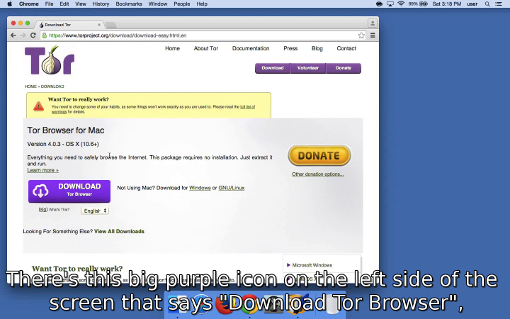
\includegraphics[width=\linewidth]{walkthrough.png}
\caption{
A participant narrates their thinking
while downloading Tor Browser.
% https://people.torproject.org/~dcf/uxsprint2015/p3.srt
{
\it
``There's this big purple icon on the left side of the screen that says `Download Tor Browser',
so I'm going to click on that because it seems like the most obvious thing.
There are a couple of other small words on the screen that I'm not going to look at, because this seems like the most obvious thing to do.''
}
}
\label{walkthrough}
\end{figure}

\indent \indent  Online artifacts of our completed pilot study, such as 
the summary, results, and resulting browser changes are below:
\begin{itemize} \itemsep1pt \parskip0pt \parsep0pt
\item \url{https://trac.torproject.org/projects/tor/wiki/org/meetings/2015UXsprint}
\item \url{https://blog.torproject.org/blog/ux-sprint-2015-wrapup}
\end{itemize}

\noindent If you would like to observe individual participants' cognitive walkthroughs, 
we transcribed the audio files from our experiment
and synced them to the screen capture we took during the duration of the experiment.
Figure~\ref{walkthrough} shows a screenshot of one of the videos.
\begin{itemize} \itemsep1pt \parskip0pt \parsep0pt
\item \url{https://people.torproject.org/~dcf/uxsprint2015/}
\end{itemize}

\subsection{Acknowledgements}
\indent \indent We thank the Tor Project for supporting the sprint, the participants, those who helped us recruit on short notice, and those who helped us plan and set goals and everyone who attended as a developer or observer: Arlo, Arthur, Ashkan, Griffin, Isis, Krishna, Mike, and Nima. We also thank the Tor help desk, whose \#tbb-helpdesk-frequent tag helped us prioritize tickets. Special thanks go to Nima for setting up the collaboration.

\section{Exit Survey Questions}
\label{sec:survey} 
\indent \indent Our participants will be taking the following exit survey, hosted through
SurveyGizmo at: 
\begin{itemize} \itemsep1pt \parskip0pt \parsep0pt
\item \url{http://www.surveygizmo.com/s3/2085559/Tor-Usability-Survey/SG_TEST_RUN}.
\end{itemize}

\noindent Recall that the survey consists of the following 17 questions, in this order: 
\begin{itemize} \itemsep1pt \parskip0pt \parsep0pt
\item 2 session and participant information questions
\item 4 basic demographics questions
\item 5 questions regarding their experience with Tor
\item 4 Internet attitude questions
\item 2 technical calibration questions
\end{itemize}

\noindent Specifically, the questions are as follows: 
\begin{enumerate} \itemsep1pt \parskip0pt \parsep0pt
\item What session did you attend?  
\item What is your participant ID? (This can be found on the sticker on the left hand corner of desk you are currently sitting at.) 
\item What is your gender? 
\item What is your age? 
\item Please select your highest level of education. 
\item What is your current occupation?*
\item How familiar were you with Tor prior to this study? 
\item Were you confident that Tor was able to provide you with security and anonymity while completing your tasks?
\item Did anything unexpected happen while using Tor?*
\item What, if any, of the following could use improvement?*
\item Based on your experience, would you use Tor again?*
\item How many hours a week would you say you spend on the internet? 
\item How concerned are you about your privacy on the Internet?
\item How concerned are you about staying anonymous on the internet?
\item How concerned are you about being censored while you browse the Internet? 
\item How familiar are you with computer security? 
\item What kinds of computer security software do you use? 
\end{enumerate}

Questions marked with asterisks are open-ended questions. All other questions are multiple choice, whether they be radio buttons, check boxes, or a drop down menu. For additional details regarding answer inputs, we refer you to our online survey linked above. 

\bibliographystyle{abbrv}
\bibliography{bibliography.bib} 
\end{document}
